\documentclass[10pt,twocolumn]{article}

\usepackage[letterpaper,margin=0.72in,columnsep=0.24in]{geometry}
\usepackage[T1]{fontenc}
\usepackage{lmodern}
\usepackage{microtype}
\usepackage{amsmath,amssymb}
\usepackage{booktabs}
\usepackage{graphicx}
\usepackage{xcolor}
\usepackage{tikz}
\usetikzlibrary{arrows.meta,positioning}
\usepackage{pgfplots}
\pgfplotsset{compat=1.18}
\usepackage[hidelinks]{hyperref}
\usepackage{url}

\definecolor{vSixBlue}{HTML}{1F77B4}
\definecolor{baseGray}{HTML}{8A8A8A}
\definecolor{tabOrange}{HTML}{E1812C}
\definecolor{softBlue}{HTML}{EAF3FA}
\definecolor{softOrange}{HTML}{FBEBDD}

\newcommand{\model}{V6}
\newcommand{\crcb}{Cr/Cb}
\newcommand{\code}[1]{\texttt{#1}}

\title{\textbf{Lightweight Residual Chroma Reconstruction from 4:2:0}}
\author{Bruno Rios\\
\small University of Texas Rio Grande Valley}
\date{August 2026}

\begin{document}
\maketitle

\begin{abstract}
Chroma subsampling reduces bandwidth by storing color at a lower spatial
resolution than luma, but conventional interpolation blurs color transitions and
can misalign them with luminance edges.  This paper studies \model, a compact
residual convolutional network that reconstructs full-resolution chroma from a
synthetic 4:2:0 observation while copying luma exactly.  The 593,794-parameter
model predicts only a two-channel correction to bilinearly upsampled chroma and
is optimized with chroma-only $\ell_1$ loss.  In a seeded paired pilot on twenty
$64\!\times\!64$ COCO crops, \model{} obtains 50.5231 dB mean chroma PSNR,
versus 47.0957 dB for bilinear interpolation and 46.8985 dB for image-adaptive
TabPFN V3.  Its paired gains are 3.4274 dB over bilinear (95\% bootstrap
confidence interval: 2.7926--4.1407 dB) and 3.6246 dB over TabPFN
(3.0489--4.2389 dB), with 20/20 wins.  An archived 3,703-image evaluation reports
a 3.88 dB chroma-PSNR gain, but lacks the original manifest.  To close that
evidence gap, this revision adds a fully local, hash-addressed protocol covering
lossless 4:4:4 sources, a $3\!\times\!4$ siting/filter matrix, actual
JPEG/H.264/HEVC/AV1 round trips, classical and learned baselines, controlled
ablations, perceptual/color metrics, resource profiling, and difficult-boundary
crops.  A repository-local 12-image procedural fixture verifies the machinery and
produces 1,024 method-image-condition records, including real H.264, HEVC, and AV1
round trips; it is explicitly not scientific evidence.  A
publication-scale rerun awaits a separately supplied local lossless corpus.
\end{abstract}

\section{Introduction}

Many image and video pipelines represent color using a luma channel $Y$ and two
chroma channels.  In 4:2:0 sampling, each chroma plane has one quarter as many
samples as luma.  Reconstructing full-resolution color is therefore a structured
missing-data problem: edges in $Y$ provide a strong spatial cue, but the missing
\crcb{} values cannot be recovered by interpolation alone.

This work asks whether that structure is better exploited by a small
convolutional refiner or by a general tabular foundation model.  The repository's
earlier V5 system used a U-Net-like generator and PatchGAN-style discriminator,
drawing on common image-to-image translation designs
\cite{ronneberger2015unet,isola2017pix2pix}.  Its adversarial objective could
produce plausible detail, but its archived pixel-fidelity scores were below
bilinear interpolation.  Version 6 instead encodes three conservative choices:

\begin{itemize}
  \setlength\itemsep{1pt}
  \item preserve the observed luma exactly;
  \item begin from a bilinear chroma estimate; and
  \item learn only the chroma residual under a direct reconstruction loss.
\end{itemize}

This paper makes three contributions.  First, it isolates and evaluates the V6
design against interpolation, V5, and an image-adaptive TabPFN V3 regressor.
Second, it introduces an executable publication protocol with immutable source
identity, disjoint splits, codec and sampling robustness tests, stronger
baselines, ablations, resource measurements, and per-image outputs.  Third, it
keeps three evidence tiers explicit: a reproducible 20-crop pilot, a large but
incompletely archived historical result, and a procedural local audit that
validates code paths but is not used to support performance claims.

\section{Related Work}

\paragraph{Classical reconstruction.}
Linear and cubic convolution filters remain important low-cost baselines; Keys'
cubic formulation is a canonical image-resampling reference
\cite{keys1981cubic}.  Edge-aware methods instead use a high-resolution guide:
joint bilateral upsampling transfers structure from that guide
\cite{kopf2007jbu}, while guided filtering assumes a local linear relation
between guide and output \cite{he2010guided}.  Because luma is available at full
resolution here, both are natural chroma baselines.  We therefore compare
nearest, bilinear, bicubic, Lanczos, guided-filter, and joint-bilateral
reconstruction under identical low-resolution samples.

\paragraph{Learned restoration and chroma guidance.}
SRCNN established a compact three-layer learned super-resolution baseline
\cite{dong2014srcnn}; EDSR later showed the value of deep residual blocks without
unnecessary normalization \cite{lim2017edsr}.  More recent restoration families
include windowed transformers such as SwinIR \cite{liang2021swinir} and
nonlinear-activation-free blocks such as NAFNet \cite{chen2022nafnet}.  Chroma
upsampling is not merely generic RGB super-resolution: Li et al.\ explicitly
used luma to guide a learned chroma upsampler for intra coding
\cite{li2017chroma}.  The revised benchmark consequently includes
chroma-adapted SRCNN and shallow NAF-style trainable controls in addition to V5
and the EDSR-like V6 residual body.

\paragraph{Compression-aware restoration.}
JPEG commonly couples transform quantization with chroma subsampling
\cite{wallace1991jpeg}; H.264/AVC, HEVC, and AV1 introduce distinct prediction,
transform, and filtering behavior \cite{wiegand2003h264,sullivan2012hevc,han2021av1}.
Approximating a codec can miss consequential implementation details, as work on
differentiable JPEG demonstrates \cite{reich2024diffjpeg}.  Learned decoders can
also target either distortion or perceptual plausibility
\cite{bahat2021explorable}.  This motivates testing actual locally encoded
bitstreams at several operating points rather than inferring codec performance
from a single synthetic operator.

\paragraph{Synthesis and general tabular priors.}
Encoder--decoder architectures such as U-Net retain multi-scale detail
\cite{ronneberger2015unet}; conditional adversarial models can encourage locally
realistic outputs \cite{isola2017pix2pix}, but realism and exact reconstruction
are different objectives.  TabPFN is a prior-data fitted network for
small-to-medium tabular prediction \cite{hollmann2025tabpfn}.  Our pilot
represents pixels as rows of spatial and luma-derived features.  This is
flexible and needs no project-specific offline training, but does not encode
translation-equivariant neighborhoods as directly as convolution.

\section{Residual Chroma Refiner}

\subsection{Synthetic 4:2:0 observation model}

Let the full-resolution image in normalized YCrCb coordinates be
$I=[Y,C]$, where $C=[C_r,C_b]$.  The degradation operator keeps $Y$ unchanged,
area-downsamples each chroma channel by two in both dimensions, and restores it
to the original size with bilinear interpolation:
\begin{equation}
  \widetilde{C}=U_{\mathrm{bilinear}}\!\left(D_{\mathrm{area}}(C)\right),
  \qquad X=[Y,\widetilde{C}].
  \label{eq:degradation}
\end{equation}
Thus all compared methods receive chroma derived from the same low-resolution
samples.  This is an idealized simulation rather than a complete codec model.

\subsection{Architecture and objective}

The refiner maps the three-channel tensor $X$ to 64 features with a $3\!\times\!3$
convolution.  Following residual optimization principles
\cite{he2016resnet}, eight blocks each apply convolution, ReLU, and convolution
before an identity addition.  A final $3\!\times\!3$ convolution predicts a
two-channel residual $R_\theta(X)$.  The reconstruction is
\begin{equation}
  \widehat{I}=\left[Y,\;\widetilde{C}+R_\theta(X)\right].
  \label{eq:model}
\end{equation}
All convolutions have unit stride and preserve resolution.  The network contains
593,794 trainable parameters and has a maximum theoretical receptive field of
$37\!\times\!37$ pixels.  Figure~\ref{fig:architecture} summarizes the dataflow.

\begin{figure*}[t]
  \centering
  \resizebox{\textwidth}{!}{%
  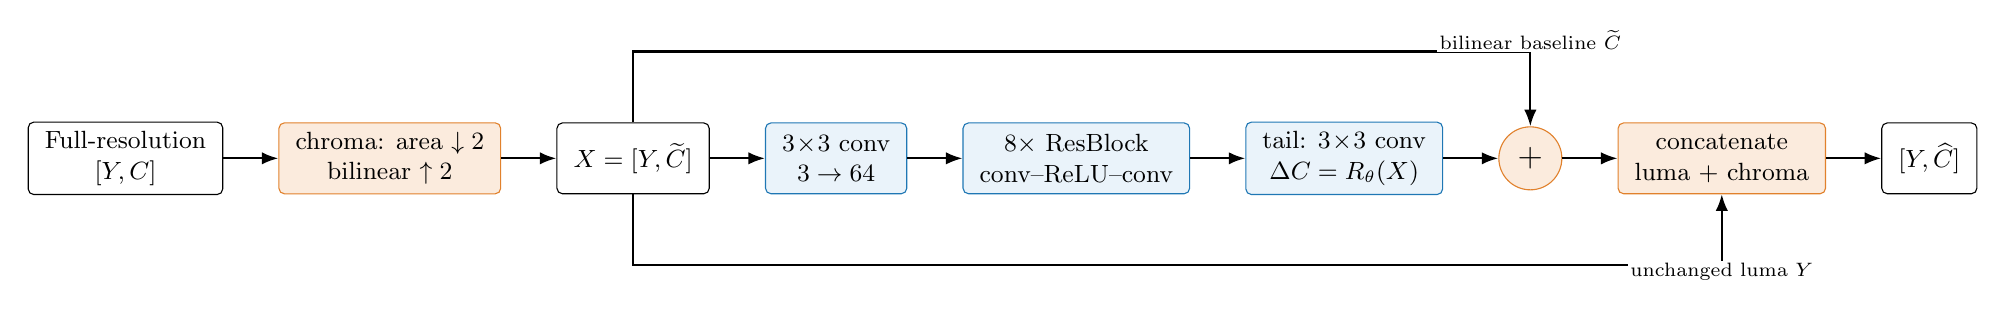
\begin{tikzpicture}[
    node distance=5mm and 7mm,
    box/.style={draw,rounded corners=2pt,minimum height=9mm,align=center,font=\small,inner xsep=6pt},
    blue/.style={box,fill=softBlue,draw=vSixBlue},
    orange/.style={box,fill=softOrange,draw=tabOrange},
    sum/.style={circle,draw=tabOrange,fill=softOrange,minimum size=8mm,inner sep=0pt,font=\large},
    arrow/.style={-{Latex[length=2.1mm]},thick}
  ]
    \node[box] (full) {Full-resolution\\$[Y,C]$};
    \node[orange,right=of full] (deg) {chroma: area $\downarrow 2$\\bilinear $\uparrow 2$};
    \node[box,right=of deg] (input) {$X=[Y,\widetilde C]$};
    \node[blue,right=of input] (head) {$3\!\times\!3$ conv\\$3\rightarrow64$};
    \node[blue,right=of head,minimum width=28mm] (body) {$8\times$ ResBlock\\conv--ReLU--conv};
    \node[blue,right=of body] (tail) {tail: $3\!\times\!3$ conv\\$\Delta C=R_\theta(X)$};
    \node[sum,right=of tail] (add) {$+$};
    \node[orange,right=of add] (assemble) {concatenate\\luma + chroma};
    \node[box,right=of assemble] (out) {$[Y,\widehat C]$};
    \draw[arrow] (full) -- (deg);
    \draw[arrow] (deg) -- (input);
    \draw[arrow] (input) -- (head);
    \draw[arrow] (head) -- (body);
    \draw[arrow] (body) -- (tail);
    \draw[arrow] (tail) -- (add);
    \draw[arrow] (add) -- (assemble);
    \draw[arrow] (assemble) -- (out);
    \draw[arrow] (input.north) -- ++(0,9mm) -|
      node[pos=0.53,above=1pt,font=\scriptsize,fill=white,inner sep=1pt]
      {bilinear baseline $\widetilde C$} (add.north);
    \draw[arrow] (input.south) -- ++(0,-9mm) -|
      node[pos=0.56,below=1pt,font=\scriptsize,fill=white,inner sep=1pt]
      {unchanged luma $Y$} (assemble.south);
  \end{tikzpicture}
  }
  \caption{Version 6 predicts a chroma correction $\Delta C$ and adds it to the
  bilinear baseline $\widetilde C$.  Luma bypasses the CNN unchanged.  Identity
  skips are also present inside every residual block.}
  \label{fig:architecture}
\end{figure*}

Training minimizes mean absolute error only on chroma:
\begin{equation}
  \mathcal{L}_{\mathrm{chroma}}(\theta)
  =\frac{1}{2HW}\left\|\widetilde{C}+R_\theta(X)-C\right\|_1.
  \label{eq:loss}
\end{equation}
The reference implementation uses random $256\!\times\!256$ crops, a 97/3
train/validation split, AdamW with learning rate $10^{-4}$, batch size 16, and 30
epochs.  Training used one NVIDIA RTX 6000 Ada GPU in a workstation equipped
with two RTX 6000 Ada GPUs.  The tested checkpoint is
\code{res\_epoch\_030.pth}.

\section{Experimental Protocol}

\subsection{Existing paired COCO pilot}

The primary completed comparison uses twenty $64\!\times\!64$ crops from COCO 2017
validation images \cite{lin2014coco}.  Sorted image paths are shuffled with seed
2026; one uniformly located crop is then drawn from each selected image.  The
same crop, color conversion, and simulated 4:2:0 observation are used for every
method.  The compared methods are bilinear interpolation, bicubic interpolation,
the epoch-10 V5 checkpoint, the epoch-30 \model{} checkpoint, and TabPFN V3.

For TabPFN, every full-resolution pixel is a test row with 16 features: normalized
coordinates; polynomial and sinusoidal coordinate terms; luma; two Gaussian
smoothings; a luma high-pass residual; horizontal and vertical luma derivatives;
and gradient magnitude.  Area-downsampled features and observed chroma form
1,024 training rows.  Two hosted regressors (identifier
\code{v3\_default}) independently predict $C_r$ and $C_b$ for 4,096 test rows.
Consequently, TabPFN is fit anew for each crop, whereas \model{} performs a
single feed-forward pass with fixed weights.

\subsection{Publication-scale data contract}

The expanded runner accepts only decoded RGB/RGBA images in lossless PNG, TIFF,
BMP, or PPM containers.  Thus every source is a full-resolution 4:4:4 raster,
not a JPEG decoded before the reference is defined.  A JSONL manifest records
the relative path, split, SHA-256 digest, dimensions, mode, format, and source
group of every image.  Hashes are recomputed before training and evaluation; an
identical digest in different splits aborts manifest creation.  Train,
validation, and test directories are physically separate, while scene-family
and near-duplicate exclusion remains an explicit curation audit.  Lossless
restoration corpora such as DIV2K provide a precedent for this source design
\cite{agustsson2017div2k}.  The full manifest must be committed before its
numbers enter the paper.

\subsection{Sampling, codecs, and baselines}

Synthetic evaluation crosses three chroma locations---centered, horizontally
left-sited, and fully cosited---with box, triangle, Gaussian, and Lanczos-3
prefilters, yielding twelve conditions.  The compared classical reconstructors
are nearest, bilinear, bicubic, Lanczos-3, guided filtering, and joint bilateral
upsampling.  Learned methods include the committed V5 and V6 checkpoints, a
retrained V6-style control, a chroma-adapted SRCNN, and a shallow NAF-style
restoration model.  All methods in a condition receive exactly the same
low-resolution chroma.

Actual codec paths complement the synthetic grid.  Pillow encodes baseline JPEG
with explicit 4:2:0 sampling at qualities 30, 50, 70, and 90.  When the requested
local FFmpeg encoders exist, H.264 and HEVC are evaluated at CRF
$\{18,23,28,35\}$ and AV1 at $\{20,30,40,50\}$, always forcing
\code{yuv420p}.  Missing executables or encoders produce structured skips.
These are single-frame round trips, so they test spatial codec artifacts but not
temporal stability.

\subsection{Controlled ablations}

Every ablation uses the same manifest, crop schedule, degradation draw, AdamW
settings, seed, and validation checkpoint rule.  Table~\ref{tab:ablations}
specifies one-factor comparisons; the SRCNN and NAF-style entries are separate
architecture controls and are not used for causal attribution.

\begin{table}[t]
  \centering
  \caption{Preregistered V6 ablation matrix.}
  \label{tab:ablations}
  \resizebox{\columnwidth}{!}{%
  \begin{tabular}{lll}
    \toprule
    Factor & Base & Alternatives \\
    \midrule
    Luma guidance & on & off \\
    Global residual & correction & direct chroma \\
    Block skips & on & off \\
    Depth (blocks) & 8 & 4, 12 \\
    Width (features) & 64 & 32, 96 \\
    Loss & $\ell_1$ & MSE, Charbonnier, $\ell_1+$edge \\
    Architecture & V6-style & SRCNN, NAF-style \\
    \bottomrule
  \end{tabular}}
\end{table}

\subsection{Metrics, statistics, and resource cost}

PSNR is computed on values normalized to $[0,1]$ and capped at 80 dB.  SSIM uses
an $11\!\times\!11$ Gaussian window \cite{wang2004ssim}.  The expanded report
contains RGB and chroma PSNR/SSIM, chroma MAE, strongest-quartile edge MAE,
gradient MAE, and mean and 95th-percentile CIEDE2000
\cite{sharma2005ciede2000}.  It also records mean/median/p95 synchronized
runtime, trainable parameters and bytes, convolutional FLOPs (a multiply and add
count as two), Python allocation peak, process-RSS delta, and accelerator
allocation peak.  Codec round-trip time and encoded bytes are labeled separately
from network inference.

Comparisons are paired by image and condition.  Mean directional differences
include win/tie rates and percentile bootstrap intervals
\cite{efron1979bootstrap}: 2,000 resamples for the existing pilot and 10,000 for
the full protocol.  Every observation is written to \code{per\_image.jsonl};
aggregates are derived from that file.  Hard examples are ranked by baseline
(bilinear or codec-native) chroma-edge error, and crops center on the strongest
reference chroma gradient.

\subsection{Evidence tiers and local audit}

The paired pilot is reproducible but small.  The separate 3,703-image record has
scale but no original manifest or per-image output, so it remains historical and
is not pooled with the pilot.  The new publication protocol is implemented but
has not been run on a natural-image corpus because none is present locally.
Instead, a repository-local procedural audit uses twelve deterministic lossless
$96\!\times\!96$ patterns split 6/2/4.  It verifies the manifest, training,
metrics, profiling, JPEG, paired aggregation, and qualitative paths.  The audit
writes 1,024 method-image-condition observations across all twelve synthetic
conditions, four JPEG qualities, and four operating points each for H.264, HEVC,
and AV1, plus 32 boundary sheets.  All 48 requested video-codec image-settings
completed through a locally installed FFmpeg, with zero skips.  These generated
patterns validate software only; no score from them is a research result.

\begin{figure*}[t]
  \centering
  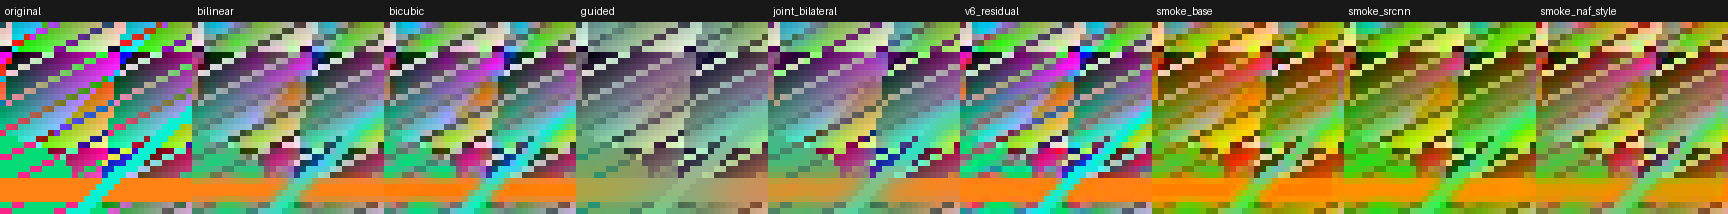
\includegraphics[width=\textwidth]{../research/reports/smoke/qualitative/center_box_bilinear_01_test_fixture_10.png}
  \caption{Automatically selected difficult-boundary crop from the procedural
  fixture audit.  Panels compare the lossless reference with classical, V6, and
  trainable smoke-model reconstructions under centered box-filtered 4:2:0.
  Nearest-neighbor display enlargement exposes chroma transitions.  The
  synthetic pattern and one-epoch smoke checkpoints make this a pipeline
  validation image, not qualitative evidence of natural-image performance.}
  \label{fig:qualitative-audit}
\end{figure*}

\section{Results}

\subsection{Paired pilot}

Table~\ref{tab:pilot} shows that \model{} has the best mean on every reported
chroma measure.  It exceeds the strongest interpolation baseline, bicubic, by
2.3658 dB and exceeds TabPFN by 3.6246 dB in chroma PSNR.  The MAE results agree
with PSNR: \model{} reduces mean chroma error by 33.8\% relative to bilinear and
27.8\% relative to TabPFN.  Its edge MAE is 39.5\% lower than bilinear and 28.8\%
lower than TabPFN, suggesting that the gain is not confined to flat regions.

\begin{table}[t]
  \centering
  \caption{Mean results on twenty paired COCO crops.  Best values are bold.
  Error metrics are lower-is-better.}
  \label{tab:pilot}
  \resizebox{\columnwidth}{!}{%
  \begin{tabular}{lrrrrr}
    \toprule
    Method & PSNR & SSIM & MAE & Edge MAE & Grad. MAE \\
    \midrule
    Bilinear & 47.0957 & 0.951135 & 0.005202 & 0.008581 & 0.002587 \\
    Bicubic  & 48.1573 & 0.959445 & 0.004745 & 0.007726 & 0.002292 \\
    V5       & 42.9576 & 0.959965 & 0.006497 & 0.008563 & 0.002380 \\
    TabPFN V3& 46.8985 & 0.961636 & 0.004773 & 0.007287 & 0.002342 \\
    \textbf{V6} & \textbf{50.5231} & \textbf{0.978180} & \textbf{0.003444} & \textbf{0.005190} & \textbf{0.001569} \\
    \bottomrule
  \end{tabular}}
\end{table}

\begin{figure}[t]
  \centering
  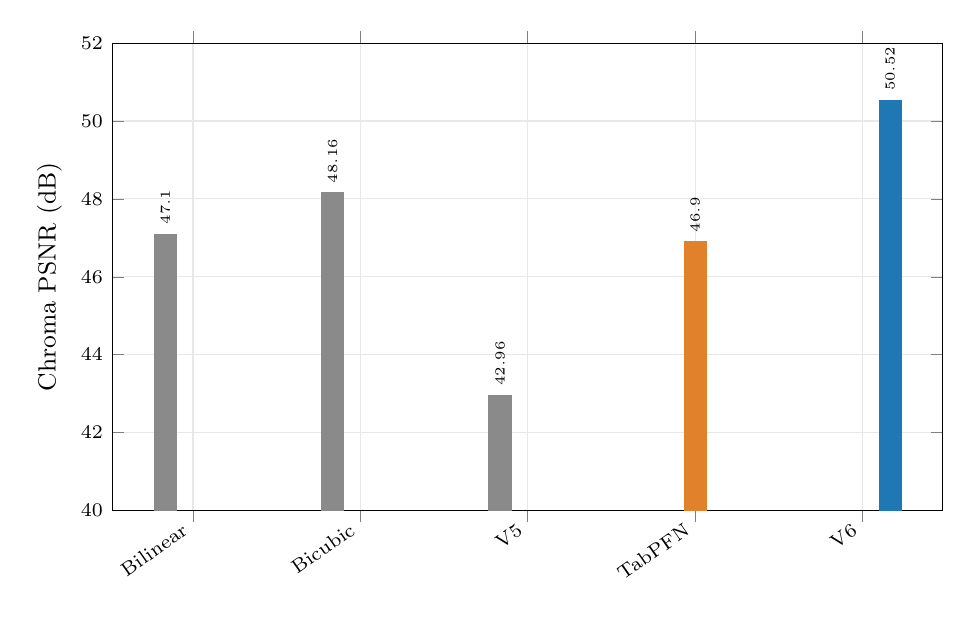
\begin{tikzpicture}
  \begin{axis}[
    ybar,
    width=\columnwidth,
    height=0.62\columnwidth,
    ymin=40,ymax=52,
    ylabel={Chroma PSNR (dB)},
    symbolic x coords={Bilinear,Bicubic,V5,TabPFN,V6},
    xtick={Bilinear,Bicubic,V5,TabPFN,V6},
    x tick label style={rotate=35,anchor=east,font=\scriptsize},
    ytick={40,42,44,46,48,50,52},
    tick label style={font=\scriptsize},
    ylabel style={font=\small},
    nodes near coords,
    nodes near coords style={font=\tiny,rotate=90,anchor=west},
    bar width=8pt,
    enlarge x limits=0.12,
    grid=major,
    grid style={draw=gray!18}
  ]
    \addplot[fill=baseGray,draw=baseGray] coordinates {
      (Bilinear,47.0957) (Bicubic,48.1573) (V5,42.9576)
    };
    \addplot[fill=tabOrange,draw=tabOrange] coordinates {(TabPFN,46.8985)};
    \addplot[fill=vSixBlue,draw=vSixBlue] coordinates {(V6,50.5231)};
  \end{axis}
  \end{tikzpicture}
  \caption{Mean chroma PSNR in the paired COCO pilot.  The truncated axis is
  labeled explicitly to emphasize method differences.}
  \label{fig:psnr}
\end{figure}

The paired analysis in Table~\ref{tab:paired} is stronger than a comparison of
means alone.  \model{} beats bilinear and TabPFN on all twenty crops in chroma
PSNR.  The confidence intervals exclude zero by wide margins.  Against TabPFN,
\model{} also wins all crops on chroma SSIM, MAE, edge MAE, and gradient MAE.

\begin{table}[t]
  \centering
  \caption{Paired chroma-PSNR advantage of \model{}.  Positive values favor
  \model{}; CIs use 2,000 bootstrap resamples.}
  \label{tab:paired}
  \begin{tabular}{lrrr}
    \toprule
    Reference & Gain (dB) & 95\% CI (dB) & Wins \\
    \midrule
    Bilinear & +3.4274 & [2.7926, 4.1407] & 20/20 \\
    TabPFN V3 & +3.6246 & [3.0489, 4.2389] & 20/20 \\
    \bottomrule
  \end{tabular}
\end{table}

TabPFN does show a different strength: relative to bilinear, it reduces average
edge MAE by 0.001293, with a 95\% interval of 0.000025--0.002893.  However, it
wins only 40\% of individual crops on that metric, and its mean chroma PSNR is
0.1972 dB lower than bilinear with an interval spanning zero.  Thus the tabular
formulation can align some chroma transitions with luma cues, but its benefit is
image-dependent in this pilot.

\subsection{Archived 3,703-image evaluation}

The larger historical record in Table~\ref{tab:archive} is consistent with the
pilot.  \model{} improves mean RGB PSNR by 3.62 dB and chroma PSNR by 3.88 dB
over bilinear interpolation.  Minimum PSNR also improves, although the 80 dB cap
is reached by both methods on some images.

\begin{table}[t]
  \centering
  \caption{Archived evaluation on 3,703 validation images.  These aggregate
  values lack a committed manifest and per-image report.}
  \label{tab:archive}
  \begin{tabular}{llrrr}
    \toprule
    Metric & Method & Mean & Min. & Max. \\
    \midrule
    RGB PSNR & Bilinear & 40.42 & 24.19 & 80.00 \\
             & V6       & \textbf{44.04} & \textbf{25.50} & 80.00 \\
    \addlinespace
    Chroma PSNR & Bilinear & 42.88 & 26.83 & 80.00 \\
                & V6       & \textbf{46.76} & \textbf{28.29} & 80.00 \\
    \bottomrule
  \end{tabular}
\end{table}

The archived video experiment reports PSNR increasing from 57.54 to 58.55 dB
and SSIM from 0.9985 to 0.9988.  Without temporal state or a committed source
video, this shows only frame-level compatibility.

\subsection{Why the conservative design helps}

Three observations explain the result.  First, copying $Y$ makes RGB fidelity
monotonic with chroma quality for a fixed conversion; the model cannot damage
already observed luminance.  Second, predicting a residual makes bilinear
interpolation an easily retained default in smooth or uncertain regions.  Third,
the convolutional body encodes locality and translation equivariance directly.
TabPFN receives engineered spatial features, but it must infer neighborhood
behavior from an unordered table and fit two regressors for every image.  The
results support the task-specific inductive bias of \model{} over a more general
tabular prior for this reconstruction setting.

The V5 comparison reinforces the loss-design argument.  V5 attains slightly
higher chroma SSIM than bilinear in the archived record (0.9536 versus 0.9530),
yet loses 1.90 dB chroma PSNR and 3.31 dB RGB PSNR.  Adversarial synthesis can
favor plausible structure without preserving the exact target samples.  For
chroma reconstruction aimed at objective fidelity, direct residual regression is
better aligned with the evaluation criterion.

\section{Limitations and Future Work}

The implementation closes the earlier protocol omissions, but not the evidence
gap by itself.  Twenty crops remain too few to characterize COCO, and their
$64\!\times\!64$ size favors manageable TabPFN tables rather than
full-resolution scaling.  The historical large result is still unauditable.
Most importantly, the new large natural-image benchmark has not been executed:
the repository contains neither a licensable lossless corpus nor the missing
historical sources.  Although all three local codec encoders complete on the
procedural fixture, substituting generated patterns for a natural corpus would
create a misleading result, so their scores remain excluded from the claims.

SHA-256 prevents exact split duplication but cannot detect altered
near-duplicates or frames from the same scene; those require corpus-level
grouping and perceptual-duplicate review.  The codec experiment processes
independent frames and decoded RGB, not native decoder chroma planes, so it
cannot establish temporal consistency or bit-exact chroma behavior.  Runtime and
memory are hardware- and backend-dependent, and the reported convolutional FLOP
count excludes non-convolutional operations.  Finally, the NAF-style control is
a shallow same-resolution adaptation, not a reproduction of the full NAFNet
encoder--decoder.

Completion now requires execution rather than further metric design: supply and
curate the local lossless corpus, commit its manifest, train the preregistered
matrix, enable the local codec encoders, run the full configuration, and commit
the per-image report and boundary crops before replacing any table.  A later
video study should add multi-frame sequences and a temporal-consistency metric.

\section{Conclusion}

A 593,794-parameter residual CNN provides a strong, simple solution to synthetic
4:2:0 chroma reconstruction.  On the paired COCO pilot, \model{} improves chroma
PSNR by 3.43 dB over bilinear interpolation and 3.62 dB over image-adaptive
TabPFN, winning every crop in both comparisons.  The archived 3,703-image result
reports a similar 3.88 dB advantage over bilinear.  These gains arise from a
useful alignment of architecture and objective: preserve luma, retain bilinear as
the base case, exploit local spatial structure, and learn only the missing color
correction.  The revised repository makes the essential next test
audit-ready---including source identity, codec diversity, strong baselines,
ablations, perceptual color error, cost, and qualitative boundaries---while
leaving publication-scale cells empty until real local data are available.

\section*{Reproducibility Statement}

The implementation and committed checkpoints are available in the
\href{https://github.com/brunorios1080/neural-chroma-reconstruction}{Neural
Chroma Reconstruction repository}.
The paired pilot is documented at revision \code{f4c8563} and is generated by
\code{scripts/benchmark\_coco\_tabpfn.py} with 20 images, crop size 64, seed
2026, the committed V5 and V6 checkpoints, hosted model identifier
\code{v3\_default}, and 2,000 bootstrap samples.  Hosted TabPFN execution requires
the corresponding client credentials.  The historical values are transcribed
from the project README and are explicitly labeled non-reproducible in this
paper.  The expanded local protocol is defined by
\code{research/configs/benchmark\_full.json} and
\code{research/configs/ablations.json}.  Its procedural audit is reproducible
from \code{research/manifests/fixture.jsonl}; outputs are stored under
\code{research/reports/smoke}, including all 1,024 JSONL records and the crop shown
in Figure~\ref{fig:qualitative-audit}.  No network service is used by that audit.

\bibliographystyle{unsrt}
\bibliography{references}

\end{document}
